\section{Propuesta}
Ya que es un tfg de desarrollo describimos lo realizado y cómo, así como los resultados obtenidos.

\subsection{Metodología}
\label{sec:metodologia}
% TODO: Explicar todo lo relacionado con la metodología en este apartado junto con la justificación de por qué se ha elegido.

Para el desarrollo de este proyecto se va a hacer uso de la metodología ágil Scrum. Esta metodología se basa en el desarrollo iterativo e incremental, lo que permite una mayor flexibilidad y adaptación a los cambios durante el proceso de desarrollo.

Se ha optado por el uso de Scrum en vez de otra metodología ágil como Kanban o XP (Extreme Programming) o alguna metodología tradicional ya que se ha utilizado anteriormente y se considera que es con la que más cómodo y eficaz se va trabajar.

Tal y como se explica en la guía oficial de Scrum \cite{scrum-guide}, Scrum es un marco de trabajo ágil que se utiliza para gestionar proyectos complejos y adaptarse a los cambios de manera rápida y eficiente. Se basa en la colaboración entre equipos multidisciplinarios, la entrega continua de valor y la mejora continua.
Scrum se centra en la entrega de incrementos de producto funcionales en ciclos cortos, lo que permite a los equipos recibir retroalimentación temprana y ajustar su enfoque según sea necesario. Esto es especialmente útil en proyectos donde los requisitos pueden cambiar con frecuencia o donde la incertidumbre es alta.

Scrum se basa en una serie de roles, eventos y artefactos que ayudan a los equipos a organizar su trabajo y colaborar de manera efectiva. Los roles incluyen el Product Owner (responsable de la visión del producto), el Scrum Master (facilitador del proceso) y el equipo de desarrollo (responsable de la entrega del producto). Los eventos incluyen las reuniones diarias, las revisiones de sprint y las retrospectivas, que permiten a los equipos reflexionar sobre su trabajo y mejorar continuamente.

Aunque, tal y como se ve, Scrum está muy enfocado a equipos, también es posible utilizarlo con un equipo muy pequeño o incluso con una sola persona, realizando los mismos eventos pero sin la necesidad de tener un equipo de desarrollo. Éste es el enfoque que se le va a dar a este proyecto. Una buena práctica de Scrum es documentar todas las reuniones y tomas de decisiones que se toman a lo largo de la vida del proyecto, ya que esto ayuda a tener una mejor organización y a poder ver cómo ha ido evolucionando el proyecto a lo largo del tiempo. Es por ello que se van a documentar todas las decisiones que se tomen y los cambios que se realicen en el desarrollo.

Tal y como se comenta en la guía de Scrum, durante el desarrollo del proyecto se van a generar varios artefactos:
\begin{itemize}
    \item \textbf{Product Backlog}: es una lista priorizada de requisitos o tareas pendientes en un proyecto ágil. En este caso, el product backlog se va a utilizar para organizar todas las historias de usuario e historias técnicas que se van a implementar en el proyecto.
    \item \textbf{Sprint Backlog}: es una lista de tareas (las cuales salen de las historias de usuario y técnicas) seleccionadas del product backlog que se van a realizar durante un sprint.
    \item \textbf{Incremento}: es la suma de todos los elementos del product backlog completados durante un sprint y los incrementos de todos los sprints anteriores. En este caso, el incremento se va a utilizar para organizar todas las tareas que se han realizado durante cada sprint.
\end{itemize}
De esta manera buscamos al tener un objetivo de producto claro y definido en los sprints. Aunque el producto sufra cambios después, queremos intentar estimar lo mejor posible y, sobre todo, terminar los sprints con un producto con \textbf{valor}, tal y como se dice en la guía `\textit{A product is a vehicle to deliver value. It has a clear boundary, known stakeholders, well-defined users or customers. A product could be a service, a physical product, or something more abstract.}'

Separaremos el desarrollo en distintos sprints, cada uno de ellos con una duración de dos semanas.

Durante cada sprint se seleccionarán las historias de usuario\footnote{Las historias de usuario son descripciones concisas y sencillas de una funcionalidad, escritas desde la perspectiva del usuario} al principio del sprint generando así el Sprint Backlog correspondiente a ese sprint, se realizarán las tareas necesarias para completarlas y al final del sprint se realizará una revisión y una retrospectiva del mismo, donde se evaluará lo que se ha hecho, cómo se puede mejorar y se planificará el siguiente sprint dependiendo del estado del recién terminado.

Gracias a esta metodología conseguimos tener una organización muy clara de lo que se va a hacer, cómo se va a hacer y cuándo se va a hacer.

\subsection{Tecnologías}
% TODO: Relacionar con los requisitos/objetivos.
Para el desarrollo de este proyecto se ha buscado utilizar tecnologías que sean lo más eficientes y rápidas posibles, pero a la vez que sean seguras y escalables. Se ha buscado un equilibrio entre rendimiento y facilidad de uso, ya que el objetivo principal es conseguir un producto funcional y eficiente.

\subsubsection{Servidor}
Para la parte de servidor se va a hacer uso de uno de los lenguajes más venerados en la actualidad en el mundo de la programación, \textbf{Rust}.

Rust es un lenguaje de programación de sistemas que se centra en la seguridad, el rendimiento y la concurrencia. Se ha convertido en una opción popular para el desarrollo de aplicaciones de alto rendimiento y sistemas críticos.
Aunque Rust es un lenguaje de bajo nivel, su sintaxis es muy similar a la de otros lenguajes de programación como C++ o Java, lo que facilita su aprendizaje para los programadores que ya tienen experiencia en estos lenguajes, permitiendo un desarrollo más seguro, rápido y eficiente. 

¿Por qué la elección de este lenguaje para el desarrollo del servidor de sincronización?
\begin{itemize}
    \item \textbf{Rendimiento}: es conocido por su alto rendimiento, lo que lo convierte en una excelente opción para aplicaciones que requieren un procesamiento intensivo de datos. Aunque es un lenguaje enfocado a sistemas, el rendimiento de sus librerías para desarrollo web es muy bueno, como se puede ver en distintos benchmark \cite{rust-benchmark}.
    \item \textbf{Seguridad}: tiene un sistema de tipos y un modelo de propiedad que ayudan a prevenir errores comunes de programación, como desbordamientos de búfer y condiciones de carrera.
    \item \textbf{Concurrencia}: soporta de manera nativa y sencilla la escritura de código concurrente y paralelo, lo que es esencial para aplicaciones que manejan múltiples tareas al mismo tiempo.
    \item \textbf{Manejo de errores}: tiene un enfoque único para el manejo de errores, utilizando tipos de datos como \texttt{Result} y \texttt{Option} para representar resultados exitosos y fallidos, lo que ayuda a evitar errores en tiempo de ejecución, consiguiendo de esta manera no encontrarnos con errores inesperados a la hora de ejecutar la aplicación.
    \item \textbf{Ecosistema}: cuenta con un ecosistema en crecimiento, con una amplia variedad de bibliotecas y herramientas que facilitan el desarrollo de aplicaciones.
\end{itemize}

Haremos uso del framework de aplicaciones web \href{https://github.com/tokio-rs/axum?tab=readme-ov-file}{\textbf{Axum}}.

Axum es un framework de aplicaciones web construido sobre Tokio, una biblioteca de programación asíncrona para Rust. Axum se centra en la simplicidad y la facilidad de uso, lo que lo convierte en una excelente opción para desarrollar aplicaciones web rápidas y eficientes.
Aunque hay varios frameworks más eficientes en términos de velocidad a la hora de realizar benchmarks\footnote{\href{https://web-frameworks-benchmark.netlify.app/result?l=rust}{Comparativa frameworks de Rust}} \footnote{\href{https://www.techempower.com/benchmarks/\#section=data-r21&test=composite&hw=ph}{Comparativa con frameworks de otros lenguajes}}, algunos de ellos tienen un tiempo de compilación demasiado alto, por lo que puede llegar a hacer más lento el desarrollo.
Además, ninguno de los demás frameworks de Rust tiene una comunidad tan activa como la de Axum ni una documentación tan completa.

Axum al estar desarrollado sobre la librería de Tokio\footnote{Librería de Rust más usada para la programación asíncrona}, garantiza un soporte a largo plazo que otros frameworks no garantizan. Además, es \href{https://lib.rs/crates/axum}{la librería más descargada }mensualmente para aplicaciones web en Rust.  

Como se puede ver en los benchmark hay frameworks de otros lenguajes que pueden parecer más sencillos que Rust que nos dan el mismo o mejor rendimiento, pero tal y como se ha comentado anteriormente, el punto principal de Rust no es únicamente su rendimiento, sino la seguridad que da el propio lenguaje y lo poco propenso que es a errores en tiempo de compilación, lo que hace de la aplicación mucho más robusta, segura y sostenible a largo plazo.


\subsubsection{Móvil}
Para el desarrollo de la aplicación móvil se ha optado por un nuevo framework de desarrollo multiplataforma, \textbf{Lynx.js}.

Lynx.js es un framework inspirado en React Native. El desarrollo de la aplicación se hace con React el cual se compila a código nativo de la plataforma. El framework soporta componentes de cualquier framework de desarrollo web, aunque está pensado para usar React y es lo que usaremos nosotros.

Aunque pueda parecer igual que React Native, Lynx añade algunas cosas que le faltan a React Native. Uno de los mayores problemas de React Native es su rendimiento en algunas situaciones, ya que este solamente hace uso de un solo thread, lo cual no permite una buena gestión de las tareas. Por ejemplo, no puede obtener datos de una API mientras que se actualiza lo que se muestra al usuario.

Sin embargo, Lynx tiene dos threads, un main thread y un background thread.
Gracias a esto, es posible especificar en qué thread se va a ejecutar cada función, consiguiendo de esta manera que tareas como mostrar rápidamente la interfaz se hagan lo más rápido posible mientras que en el background thread se obtienen los datos de la API.
Esto da una experiencia al usuario mucho más fluida y rápida, principalmente gracias a el \textit{Instant First-Frame Rendering (IFR)}\footnote{El \href{https://lynxjs.org/guide/interaction/ifr.html}{Instant First-Frame Rendering (IFR)} es una técnica de renderizado que permite mostrar el primer fotograma de una aplicación de manera instantánea, mejorando la experiencia del usuario al reducir el tiempo de espera para ver la interfaz.}.

Para conseguir esto, Lynx altera el ciclo de vida de los componentes de React (figura \ref{fig:lynx-component-lifecycle}), consiguiendo deshacerse de cuellos de botella típicos que aparecen en los frameworks de desarrollo móvil asegurando un rendimiento óptimo y una experiencia de usuario fluida.

\begin{figure}[h]
    \begin{center}
        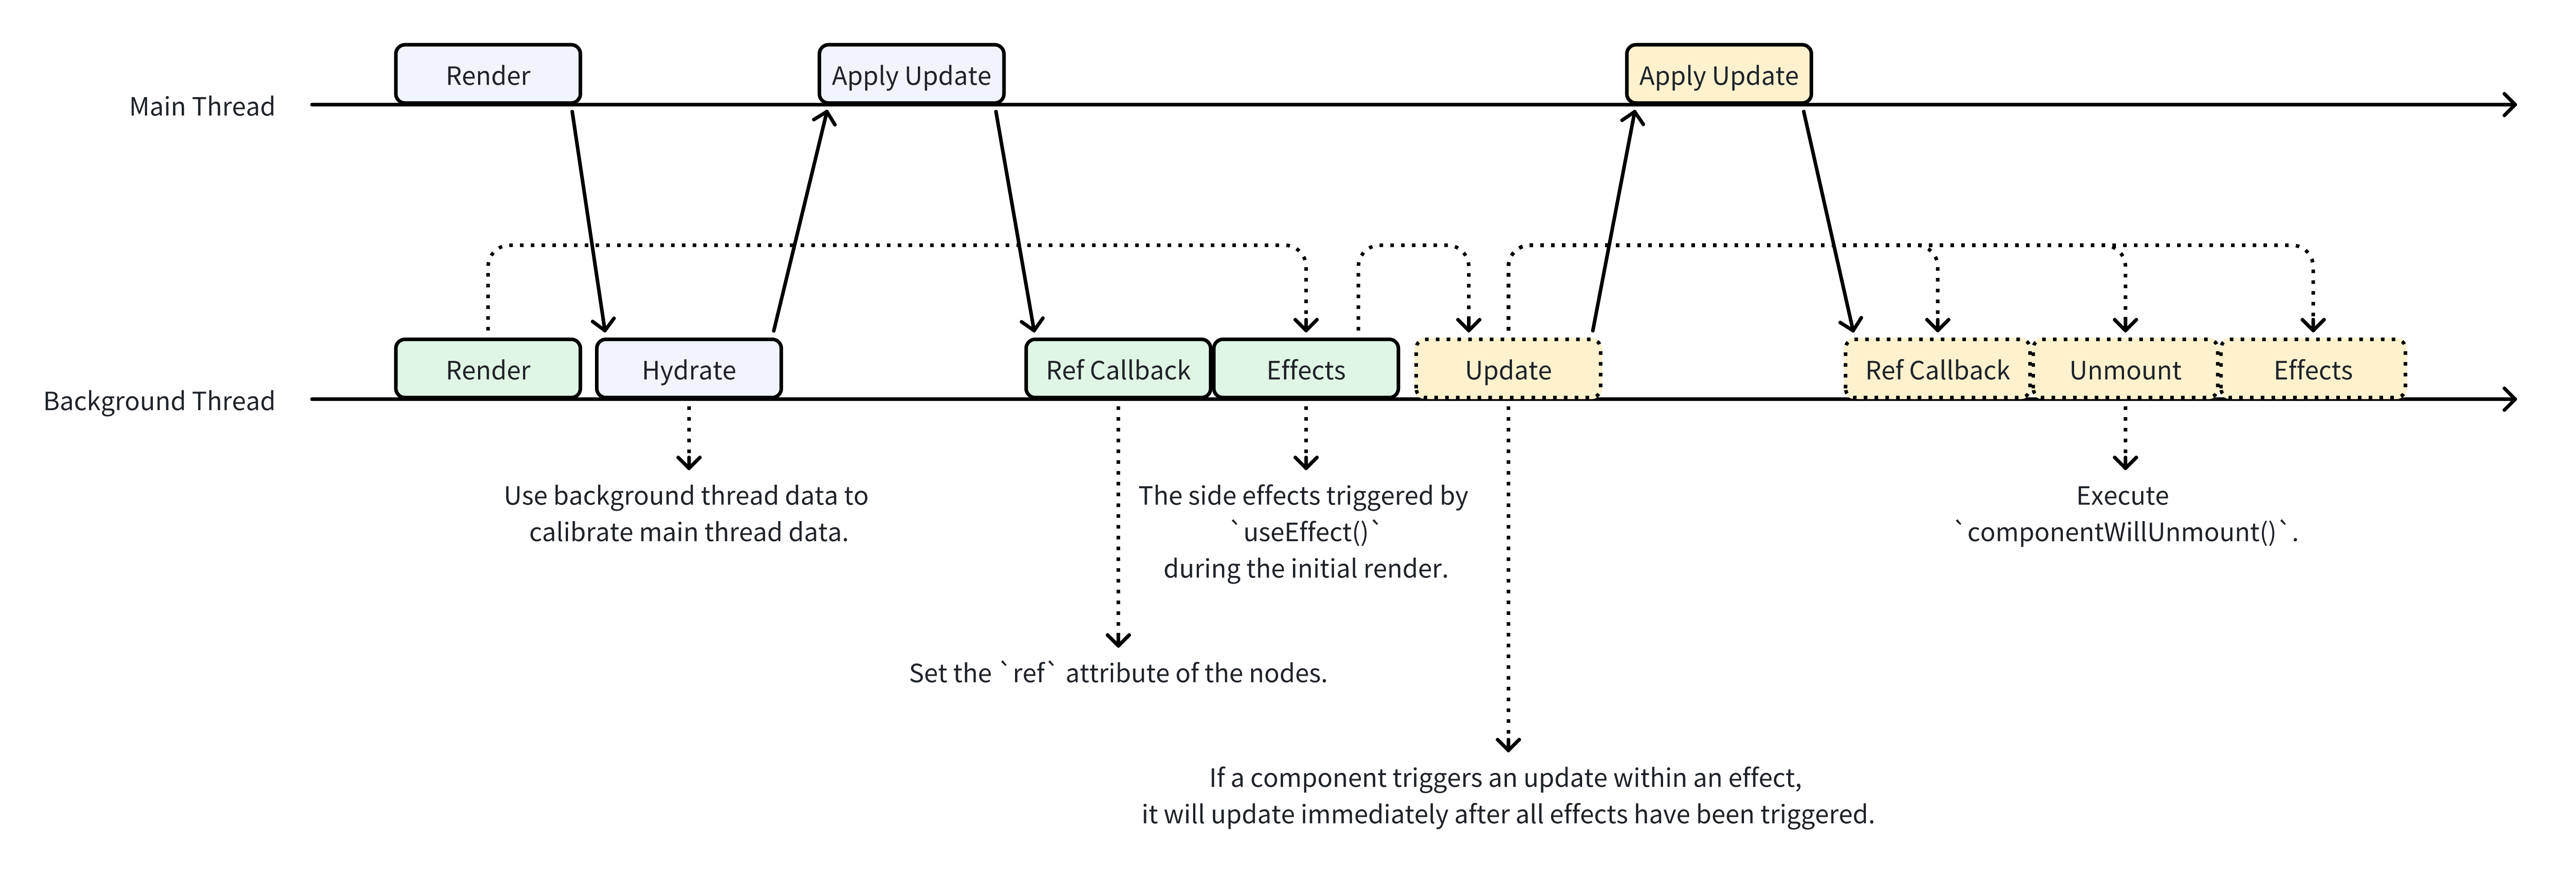
\includegraphics[width=\textwidth]{lynx-lifecycle.png}
    \end{center}
    \caption{Ciclo de vida de los componentes en Lynxjs (\href{https://lynxjs.org/react/lifecycle.html}{Documentación})}
    \label{fig:lynx-component-lifecycle}
\end{figure}


Dado que la aplicación necesitará hacer uso de módulos nativos de los teléfonos, necesitaremos implementarlos para cada plataforma.
Esto se puede hacer de manera sencilla, ya que el framework permite la creación de módulos nativos los cuales se pueden llamar desde nuestro código escrito en React.

Este es uno de los puntos fuertes de la aplicación, ya que nos va a permitir programar haciendo uso de React, el cual es un framework muy conocido y utilizado, pero a la vez nos va a permitir hacer uso de módulos nativos de cada plataforma, lo que nos da una gran flexibilidad a la hora de desarrollar la aplicación de forma nativa en todas las plataformas.

Lynx usa una aplicación nativa \textit{Lynx Explorer}, con la cual podemos ver cómo se va a ver la aplicación en el dispositivo móvil. Esta aplicación es la que se encarga de compilar el código de Lynx a código nativo y de ejecutar la aplicación en el dispositivo móvil.
Para poder hacer uso de los módulos nativos, tendremos que implementarlos en el Explorer, compilar el código del mismo y una vez tenemos la aplicación con nuestro módulo nativo, podemos ejecutar nuestra aplicación sobre el Explorer y hacer uso de nuestro módulo nativo.

Todo esto, junto con los comandos y repositorios necesarios viene detallado en el artículo hecho por el equipo de Lynx \cite{lynx-native-modules}.

Dado que para el desarrollo de aplicaciones en iOS es necesario tener un sistema de Apple, en la implementación de esta aplicación nos centraremos en la parte de Android, aunque el código de la aplicación será el mismo para ambas plataformas.
La única diferencia será la implementación de los módulos nativos, que serán diferentes para cada plataforma.

En resumen, las ventajas de usar este framework con respecto a otros son:
\begin{itemize}
    \item \textbf{Rendimiento}: al compilar a código nativo, el rendimiento es mucho mejor que el de otros frameworks como Flutter. Además, Lynx nos permite hacer uso de su tecnología de doble thread, haciendo que nuestra aplicación sea mucho más fluida y rápida en comparación con otras tecnologías.
    \item \textbf{Flexibilidad}: permite la creación de módulos nativos para cada plataforma, lo que da una gran flexibilidad a la hora de desarrollar la aplicación.
    \item \textbf{Simplicidad}: la sintaxis es muy similar a la de React, lo que facilita su aprendizaje para los programadores que ya tienen experiencia en este framework.
    \item \textbf{Documentación}: la documentación es muy completa y está en constante actualización.
\end{itemize}

¿Por qué no se ha optado por otras opciones como Flutter o Kotlin Multiplatform?
\begin{itemize}
    \item \textbf{Flutter}: aunque es un framework muy potente y con una comunidad muy activa, su rendimiento no es tan bueno como el de Lynx.js. 
        Flutter lo que hace es renderizar lo que sería como un "canvas" que utiliza un motor gráfico parecido al de los juegos para renderizar la interfaz de usuario, haciendo que la experiencia de usuario no sea tan fluida como podría ser la de otro framework. 
    \item \textbf{Kotlin Multiplatform}: aunque es una opción interesante, la comunidad y la documentación son mucho más limitadas que las de Lynx.js. La curva de aprendizaje es mucho más pronunciada, ya que se utiliza Kotlin junto con una gran cantidad de librerías las cuales necesitan de un estudio profundo para su uso.

        Nos daría el mejor rendimiento sin tener que programar la aplicación de forma nativa para todos los dispositivos (los dispositivos comparten código pero hay que implementar la mayoría de forma nativa para las distintas plataformas), pero el desarrollo sería mucho más lento y tedioso, lo cual además complicaría la aportación al proyecto Open Source.
    \item \textbf{React Native}: aunque es un framework muy conocido y utilizado, su rendimiento no es tan bueno como el de Lynx.js.
        Es una opción muy parecida a Lynx.js, pero a largo plazo la aplicación podría verse afectada por el rendimiento.
        Dada la similitud con Lynx.js y las ventajas que ofrece, se ha optado por este último.
\end{itemize}

Este framework ha sido desarrollado de cero por el equipo de TikTok. Es utilizado por ellos para el desarrollo de varias de sus aplicaciones, por lo que aunque ha cambiado a ser Open-Source hace poco con su versión 3.2.0, es un framework que ya ha sido probado en producción en aplicaciones como \textbf{TikTok Studio}, \textbf{Disney100 en TikTok}, \textbf{The Met Gala en TikTok} tal y como comentan en el artículo en el que anunciaron que Lynxjs pasaba a ser Open-Source \cite{lynx-article}.

\subsection{Historias de usuario / Historias técnicas}
En esta sección se detallan las historias de usuario e historias técnicas de la aplicación, separadas en dos grupos: las de la aplicación de servidor y las de móvil.

Se ha considerado esta separación ya que la aplicación de servidor tiene un objetivo diferente al de la aplicación móvil, de esta manera conseguimos una mejor organización de las historias de usuario.

Durante los primeros sprints se trabajará de manera principalmente separada, enfocándose en la parte correspondiente que se defina de la aplicación y en una fase más avanzada se trabajará de manera conjunta, integrando ambas aplicaciones. Esto lo hacemos para para poder enfocarnos mejor en una sola parte del proyecto, de esta manera no tenemos que estar cambiando de contexto constantemente entre las dos aplicaciones, lo que podría hacer que el desarrollo fuera más lento y tedioso.

Para la planificación del desarrollo se han utilizado puntos de historia (PH), los cuales representan una estimación de lo que se considera que se tardará en implementar las historias de usuario. Esta estimación es relativa, es decir, no representa un tiempo real sino una estimación con respecto a todas las demás historias de usuario, siendo 1 punto de historia la historia de usuario más sencilla de implementar o que menos tiempo requiere.

Este es un listado inicial de historias de usuario, durante los sprints se irá especificando si alguna historia de usuario ha cambiado, añadido o eliminado del product backlog\footnote{El product backlog es una lista priorizada de requisitos o tareas pendientes en un proyecto ágil.}.

Cada historia de usuario tiene un identificador único, una descripción de la historia de usuario y una estimación en puntos de historia. Ésta es después desglosada en historias de usuario más pequeñas de las cuales se definen tareas que tienen que ser realizadas para completar la historia de usuario con su estimación en horas.
Además de las historias de usuario, contamos con historias técnicas, que son historias de usuario que no están relacionadas directamente con el usuario final, sino que son necesarias para el correcto funcionamiento del sistema. Estas historias técnicas se consideran como historias de usuario y se les asigna una estimación en puntos de historia.

A lo largo del product backlog  se hará referencia a HU\{identificador\} para las historias de usuario y HT\{identificador\} para las historias técnicas. El identificador será un número entero que se asignará de manera consecutiva a cada historia de usuario o historia técnica. Para la sub-historias de usuario se asignará un número entero que será el mismo que la historia de usuario a la que pertenece, seguido de un punto y otro número entero que será el identificador de la sub-historia de usuario, por ejemplo: HU1, HU1.1, HU1.2, etc.

\subsubsection{Servidor}
\renewcommand{\arraystretch}{1.3} % Increases row height for readability
\rowcolors{2}{gray!15}{white} % Alternate row colors

\begin{tabularx}{\textwidth}{|l|l|>{\raggedright\arraybackslash}X|p{2cm}|}
    \hline
    \textbf{ID} & \textbf{Título} & \textbf{Descripción} & \textbf{Estimación (PH)} \\
    \hline
    HU01 & Subida de fotos & Como usuario, quiero subir varias fotos desde mi móvil para tener una copia de seguridad en mi servidor. & 5 \\
    \hline
    HU02 & Estado de sincronización & Como usuario, quiero ver qué fotos están subidas y cuáles no, para saber el estado de sincronización. & 3 \\
    \hline
    HU03 & Eliminar fotos & Como usuario, quiero eliminar fotos subidas desde la app, para liberar espacio en mi servidor. & 3 \\
    \hline
    HU04 & Subida de vídeos & Como usuario, quiero subir vídeos además de fotos, para guardar también mis recuerdos en vídeo. & 5 \\
    \hline
    HU05 & Inicio de sesión & Como usuario, quiero iniciar sesión con contraseña o clave, para evitar que otros accedan a mis archivos. & 5 \\
    \hline
    HU06 & Cerrar sesión & Como usuario, quiero poder cerrar sesión en un dispositivo, para proteger mis datos si pierdo el móvil. & 2 \\
    \hline
    HU07 & Descubrimiento automático & Como usuario, quiero que la app detecte automáticamente mi servidor en la red local, para no tener que configurarlo manualmente. & 8 \\
    \hline
    HU08 & Conexión remota & Como usuario, quiero poder conectarme remotamente si expongo mi servidor, para acceder a mis fotos desde fuera de casa. & 13 \\
    \hline
    HU09 & Galería visual & Como usuario, quiero ver una galería de las fotos subidas, para revisar mi contenido fácilmente. & 5 \\
    \hline
    HU10 & Espacio ocupado & Como usuario, quiero ver el espacio ocupado por mis archivos, para controlar el almacenamiento del servidor. & 3 \\
    \hline
    HU11 & Estadísticas de copia & Como usuario, quiero ver estadísticas de sincronización, para saber cuándo fue la última copia y cuántos archivos se han guardado. & 3 \\
    \hline
    HU12 & Cancelar sincronización & Como usuario, quiero cancelar una sincronización en curso. & 5 \\
    \hline
    HU13 & Crear cuentas & Como administrador, quiero crear cuentas de usuario con permisos, para que varias personas puedan usar el servidor. & 8 \\
    \hline
    HU14 & Galería privada & Como usuario, quiero tener mi propia galería separada de otros usuarios. & 5 \\
    \hline
    HU15 & Galería online & Como usuario, quiero poder ver todas las fotos que tengo en el servidor sin necesidad de tener que descargarlas en mi móvil, tanto las que he subido yo como las que han compartido conmigo. & 8 \\
    \hline
    HT01 & Hash de archivos & Implementar sistema de cálculo de hash para detectar duplicados. & 3 \\
    \hline
    HT02 & Sincronización incremental & Implementar sincronización basada en metadatos (fecha, tamaño, hash). & 5 \\
    \hline
    HT03 & API REST en Rust & Diseñar API RESTful para subida, borrado y consulta de archivos. & 13 \\
    \hline
    HT04 & Descubrimiento mDNS & Crear sistema de descubrimiento automático usando mDNS. & 8 \\
    \hline
    HT05 & Autenticación JWT & Implementar autenticación con JSON Web Tokens. & 5 \\
    \hline
    HT06 & HTTPS en servidor & Configurar comunicación segura con HTTPS. & 5 \\
    \hline
    HT07 & Estructura de almacenamiento & Definir carpetas y metadatos para organizar los archivos. & 5 \\
    \hline
    HT08 & Base de datos & Implementar SQLite o PostgreSQL para usuarios y archivos. & 8 \\
    \hline
    HT09 & Compresión de imágenes & Implementar compresión para optimizar el almacenamiento. & 5 \\
    \hline
    HT10 & Subida concurrente & Soporte para subida simultánea y manejo de errores. & 8 \\
    \hline
    HT11 & Tests en Rust & Añadir pruebas unitarias e integración en backend. & 5 \\
    \hline
    HT12 & CI/CD & Configurar pipelines de integración y despliegue. & 5 \\
    \hline
    HT13 & Logging & Implementar logs detallados para depuración. & 3 \\
    \hline
    HT14 & Cobertura de tests & Medir y asegurar la cobertura de pruebas. & 3 \\
    \hline
    HT15 & Interfaz Tauri & Crear interfaz gráfica del servidor con Tauri. & 8 \\
    \hline
    HT16 & Panel de control & Implementar visualización de archivos y uso del sistema. & 5 \\
    \hline
    HT17 & Notificaciones de progreso & Integrar notificaciones del sistema con progreso de subida. & 3 \\
    \hline
    HT18 & Binario y Tauri & Empaquetar servidor como CLI y app Tauri. & 5 \\
    \hline
    HT19 & Dockerización & Crear imagen Docker del servidor. & 3 \\
    \hline
    HT20 & Documentación & Documentar instalación y uso del sistema. & 13 \\
    \hline
    HT21 & Backups externos & Soporte para backups automáticos externos. & 8 \\
    \hline
    HT22 & Logs persistentes & Configurar sistema de logs persistentes y rotación. & 3 \\
    \hline
\end{tabularx}

\subsubsection{Móvil} 
\begin{tabularx}{\textwidth}{|l|l|>{\raggedright\arraybackslash}X|p{2cm}|}
    \hline
    ID & Título & Descripción & Estimación \\
    \hline
    HU01 & Seleccionar fotos & Como usuario, quiero seleccionar varias fotos desde mi galería para subirlas al servidor. & 3 \\
    \hline
    HU02 & Subir fotos automáticamente & Como usuario, quiero que se suban automáticamente las nuevas fotos que hago, sin tener que hacerlo manualmente. & 8 \\
    \hline
    HU03 & Ver progreso de subida & Como usuario, quiero ver el progreso de cada archivo que se está subiendo. & 8 \\
    \hline
    HU04 & Cancelar subida & Como usuario, quiero cancelar una subida en curso desde la interfaz. & 3 \\
    \hline
    HU05 & Ver archivos subidos & Como usuario, quiero ver una lista o galería de los archivos que ya están subidos. & 5 \\
    \hline
    HU06 & Conexión automática al servidor & Como usuario, quiero que la app detecte y se conecte automáticamente al servidor en mi red. & 5 \\
    \hline
    HU07 & Cambiar de servidor & Como usuario, quiero poder cambiar manualmente la dirección del servidor si quiero usar otro. & 3 \\
    \hline
    HU08 & Ver uso de almacenamiento & Como usuario, quiero ver cuánto espacio he usado en el servidor. & 3 \\
    \hline
    HU09 & Inicio y cierre de sesión & Como usuario, quiero iniciar y cerrar sesión para proteger mis datos. & 5 \\
    \hline
    HU10 & Gestión de permisos & Como usuario, quiero que la app me pida permisos de acceso solo cuando sea necesario. & 3 \\
    \hline
    HU11 & Notificaciones de subida & Como usuario, quiero recibir notificaciones cuando se complete la sincronización. & 5 \\
    \hline
    HU12 & Subir vídeos & Como usuario, quiero subir también vídeos de mi galería al servidor. & 5 \\
    \hline
    HU13 & Subida en segundo plano & Como usuario, quiero que las subidas continúen aunque cierre la app. & 8 \\
    \hline
    HU15 & Sincronización manual & Como usuario, quiero poder iniciar la sincronización manualmente. & 3 \\
    \hline
    HU16 & Galería online & Como usuario, quiero ver mis fotos en la app sin tener que descargarlas. & 5 \\
    \hline
    HT01 & Acceso a la galería & Implementar acceso seguro a la galería de fotos y vídeos. & 5 \\
    \hline
    HT02 & Comunicación con API & Integrar cliente HTTP que se comunique con el servidor. & 5 \\
    \hline
    HT03 & Almacenamiento local & Guardar estado de archivos subidos/no subidos de forma local. & 3 \\
    \hline
    HT04 & Manejo de errores de red & Implementar gestión de errores de red y reintentos automáticos. & 5 \\
    \hline
    HT05 & Subida concurrente & Soportar subida de varios archivos en paralelo con control de errores. & 5 \\
    \hline
    HT06 & Sincronización de fondo & Implementar sincronización en segundo plano. & 8 \\
    \hline
    HT07 & Pruebas unitarias & Añadir pruebas unitarias y de integración a la lógica común en React Native / Lynxjs & 13 \\
    \hline
    HT08 & CI/CD móvil & Pipeline de construcción y publicación para Android e iOS. & 5 \\
    \hline
    HT09 & Gestión de tokens & Almacenar y renovar tokens de autenticación de forma segura. & 3 \\
    \hline
    HT10 & Notificaciones locales & Integrar sistema de notificaciones locales en Android/iOS. & 3 \\
    \hline
    HT11 & Optimización de red & Reducir uso de red usando compresión. & 5 \\
    \hline
    HT12 & Localización & Soporte multilenguaje para la aplicación. & 8 \\
    \hline
    HT13 & Permisos condicionales & Solicitar permisos en tiempo de ejecución de forma contextual. & 3 \\
    \hline
    HT14 & UI responsive & Adaptar UI para distintos tamaños de pantalla (tablet, móvil). & 3 \\
    \hline
\end{tabularx}


\subsection{Planificación inicial}
Este apartado se considera como el que sería el sprint 0. Durante un desarrollo con Scrum, tal como se ha comentado anteriormente en la \hyperref[sec:metodologia]{sección de metodología}, se usan \textbf{sprints} para dividir el desarrollo en partes organizadas y planificadas con anterioridad.

Se suele crear un sprint denominado ``0'' en el que se hace una planificación inicial, se genera la que va a ser la primera versión del product backlog y se dan unas estimaciones de las tareas que se van a realizar en todos los sprints.

Además, en este sprint vamos a plantear una arquitectura inicial abstracta de nuestro sistema, la cual nos servirá como base para el desarrollo de la aplicación. Esta arquitectura se irá modificando e iterando a lo largo del desarrollo del proyecto, pero nos servirá como guía inicial para el desarrollo para definir nuestras historias de usuario y organizar de una manera correcta los sprints.

\subsection{Presupuesto}

